\begin{figure}[t]
    \centering
    \begin{minipage}[t]{0.217\linewidth}
        \centering
        \vspace{0pt}
        \vspace{0.08\linewidth}
        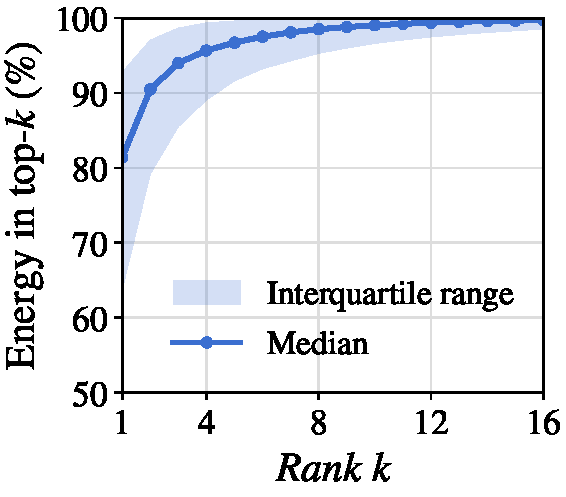
\includegraphics[width=\linewidth]{figures/state_energy.pdf}\\[0.17\linewidth]
        \caption{\protect\raggedright Energy of the top singular values in the Qwen3.5-9B model.}
        \vspace{-1.5em}
        \label{fig:energy}
    \end{minipage}%
    \hfill
    \begin{minipage}[t]{0.753\linewidth}
        \centering
        \vspace{0pt}
        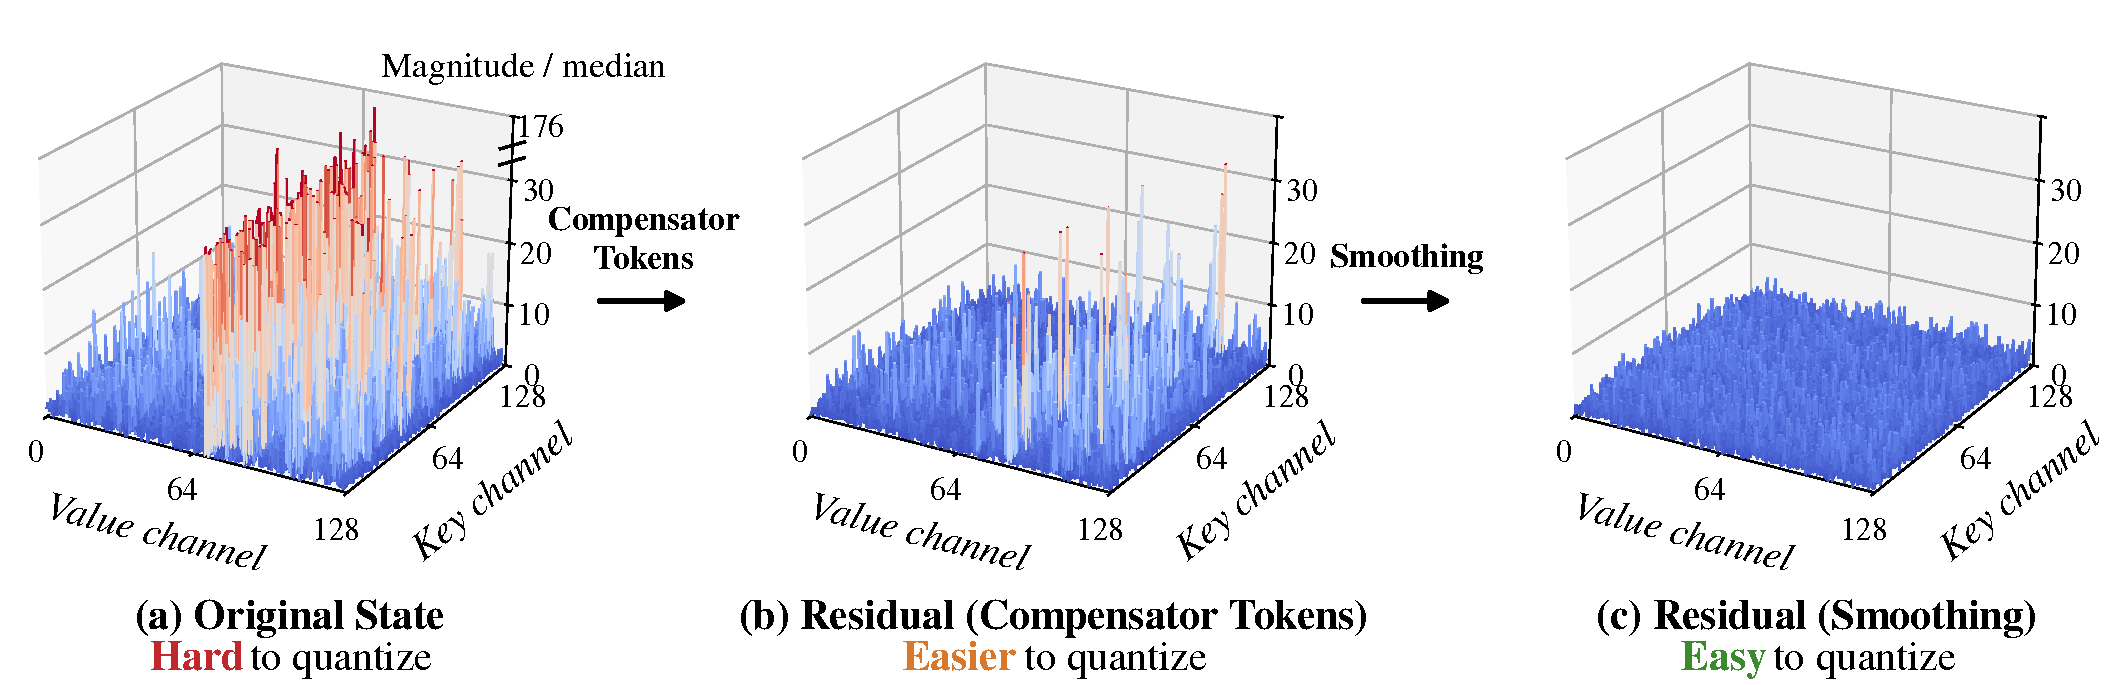
\includegraphics[width=\linewidth]{figures/state_3d.pdf}
        \caption{Magnitude of one Qwen3.5-9B head (layer 13, head 16) at 8K context, normalized by the median magnitude of $S$ in (a) and (b) and of the smoothed residual in (c).
        Outliers up to 176$\times$ the median (a) drop to 47$\times$ after Compensator Tokens (b) and to 5.3$\times$ after smoothing (c).}
        \vspace{-1.5em}
        \label{fig:state-heat}
    \end{minipage}
\end{figure}
